\documentclass[10pt,aspectratio=169,dvipsnames]{beamer}
\usetheme[]{Berlin}

\setbeamertemplate{footline}{
  \usebeamercolor[fg]{framesource}%
  \usebeamerfont{page number in head}%
  \hspace{0.2cm}
  \small \insertframenumber
  \vspace{0.2cm}
  \doclicenseIcon
  \hfill
  
\includegraphics[height=0.8cm]{graphics/logos/tub_logo.pdf}
  \hspace{0.2cm}
}

\setbeamercovered{transparent}

% wider right margin so content doesn't run into the footer logo
\setbeamersize{text margin left=1cm, text margin right=1.8cm}

% "ONGOING WORK" label along the right edge of every page
\AddToHook{shipout/foreground}{%
  \put(\paperwidth-0.45cm,-0.5\paperheight){%
    \makebox[0pt][c]{\rotatebox{90}{\makebox[0pt][c]{%
      \color{black!25}\fontsize{8}{8}\selectfont\bfseries ONGOING WORK}}}}}

\setbeamertemplate{footline}[
 myframe number]

% PACKAGES
\usepackage[absolute,overlay]{textpos}
\usepackage[utf8]{inputenc}
\usepackage[official]{eurosym}
\usepackage{booktabs,multicol,multirow,tabularx,array}
\usepackage{subcaption}
\usepackage{parskip}
\usepackage{bm}
\usepackage{tikz}
\usepackage{adjustbox}
\usepackage[super]{nth}
\usepackage[version=4]{mhchem}
\usepackage{siunitx}
\usepackage{tikz}
\usetikzlibrary{calc}


\sisetup{
  detect-all = true
}


\usepackage[
    type={CC},
    modifier={by},
    version={4.0},
]{doclicense}

% HYPERREFERENCES
\usepackage{hyperref}
\hypersetup{
	colorlinks=true,
	citecolor=tub-blue,
	linkcolor=tub-blue,
	urlcolor=tub-blue
}

\usepackage[sfdefault]{roboto}
\usepackage[normalem]{ulem}

% \usepackage[backend=biber,style=numeric-comp]{biblatex}
% \addbibresource{references.bib}

\newcolumntype{R}[1]{>{\raggedleft\arraybackslash}p{#1}}


% GRAPHICS
\graphicspath{
    {graphics/},
  }
\DeclareGraphicsExtensions{.pdf,.jpeg,.png,.jpg}

% FORMATTING
\setlength{\parskip}{6pt}
\linespread{1.1}
\newcommand{\seprule}{\par\noindent\textcolor{black!25}{\rule{\textwidth}{0.4pt}}}

% SOURCES
\setbeamercolor{framesource}{fg=gray}
\setbeamerfont{framesource}{size=\tiny}
\newcommand{\source}[1]{\begin{textblock*}{10cm}(3.6cm,8.25cm)
    \begin{beamercolorbox}[ht=0.5cm,right]{framesource}
        \usebeamerfont{framesource}\usebeamercolor[fg]{framesource} Source: {#1}
    \end{beamercolorbox}
\end{textblock*}}

% REFERENCES
% \usepackage[style=nature, doi=true, maxcitenames=3]{biblatex}
% \bibliography{bibliography}
% \renewcommand*{\bibfont}{\footnotesize}

% COLOR TEXT
\newcommand{\bl}[1]{\textcolor{tub-blue}{#1}}
\newcommand{\gr}[1]{\textcolor{tub-green}{#1}}
\newcommand{\rd}[1]{\textcolor{tub-red}{#1}}
\newcommand{\yl}[1]{\textcolor{tub-yellow}{#1}}
% \newcommand{\org}[1]{\textcolor{tub-orange}{#1}}
\newcommand{\cb}[1]{\colorbox{gray!20}{#1}}

\usepackage{array}% https://ctan.org/pkg/array
\makeatletter
\g@addto@macro{\endtabular}{\rowfont{}}% Clear row font
\makeatother
\newcommand{\rowfonttype}{}% Current row font
\newcommand{\rowfont}[1]{% Set current row font
   \gdef\rowfonttype{#1}#1%
}
\newcolumntype{L}{>{\rowfonttype}l}

\usepackage[most]{tcolorbox}
\tcbuselibrary{listingsutf8}

% Custom commands
\usepackage{caption}
\renewcommand{\figurename}{} % Removes the "Figure" text
\captionsetup[figure]{labelformat=empty, labelsep=none} % Removes numbering and colon


% FONT
%\usepackage{utopia}

% REFERENCES
%\usepackage[backend=biber,style=authoryear-comp]{biblatex}
%\bibliography{references.bib}

% DECK-SPECIFIC
\usepackage{fontawesome5}
\colorlet{ink}{black}
\colorlet{mute}{black!60}
\colorlet{rule}{black!25}
\colorlet{inv}{tub-blue}
\colorlet{adv}{tub-red}
\colorlet{rec}{tub-green}
\colorlet{panel}{tub-blue!8}

% take-away line under a figure
\newcommand{\takeaway}[1]{%
  \par\smallskip
  \colorbox{panel}{\parbox{\dimexpr\linewidth-2\fboxsep}{\footnotesize\strut#1\strut}}}

% placeholder box: \placeholder{width}{height}{text}
\newcommand{\placeholder}[3]{%
  \tikz{\node[draw=mute,dashed,thick,fill=panel,rounded corners=2pt,minimum width=#1,
    minimum height=#2,text width=\dimexpr#1-0.4cm\relax,align=center,font=\scriptsize\color{mute}]
    {\faImage\ \textbf{Placeholder}\\[0.2em]#3};}}

% TITLE PAGE
\title{
  \textbf{The cost of self-sufficiency: Robust energy system planning under prolonged
  transmission blackouts}
}
\vspace*{-.5cm}

\institute[Technische Universität Berlin] % (optional, but mostly needed)
{
  \normalsize
  \alert{ECEMP 2026 --- Session on `Energy security and geopolitical risks'} \\
  \footnotesize
  Bobby Xiong, Iegor Riepin, Tom Brown \\
  Department of Digital Transformation in Energy Systems, Technische Universität Berlin \\
  \href{mailto:xiong@tu-berlin.de}{xiong@tu-berlin.de} \\
  \vspace{0.3cm}

  21 October 2026
}

\date{}

\subject{ECEMP 2026}

\titlegraphic{%
\vspace{-1cm}

\includegraphics[height=1cm,clip=true]{graphics/logos/cetp_logo.png}
\hspace{0.5cm}
\includegraphics[height=1cm,clip=true]{graphics/logos/ensys_short_logo.pdf}
\hspace{0.5cm}
\includegraphics[trim=0 0cm 0 0cm,height=1cm,clip=true]{graphics/logos/tub_logo.pdf}
\hspace{0.5cm}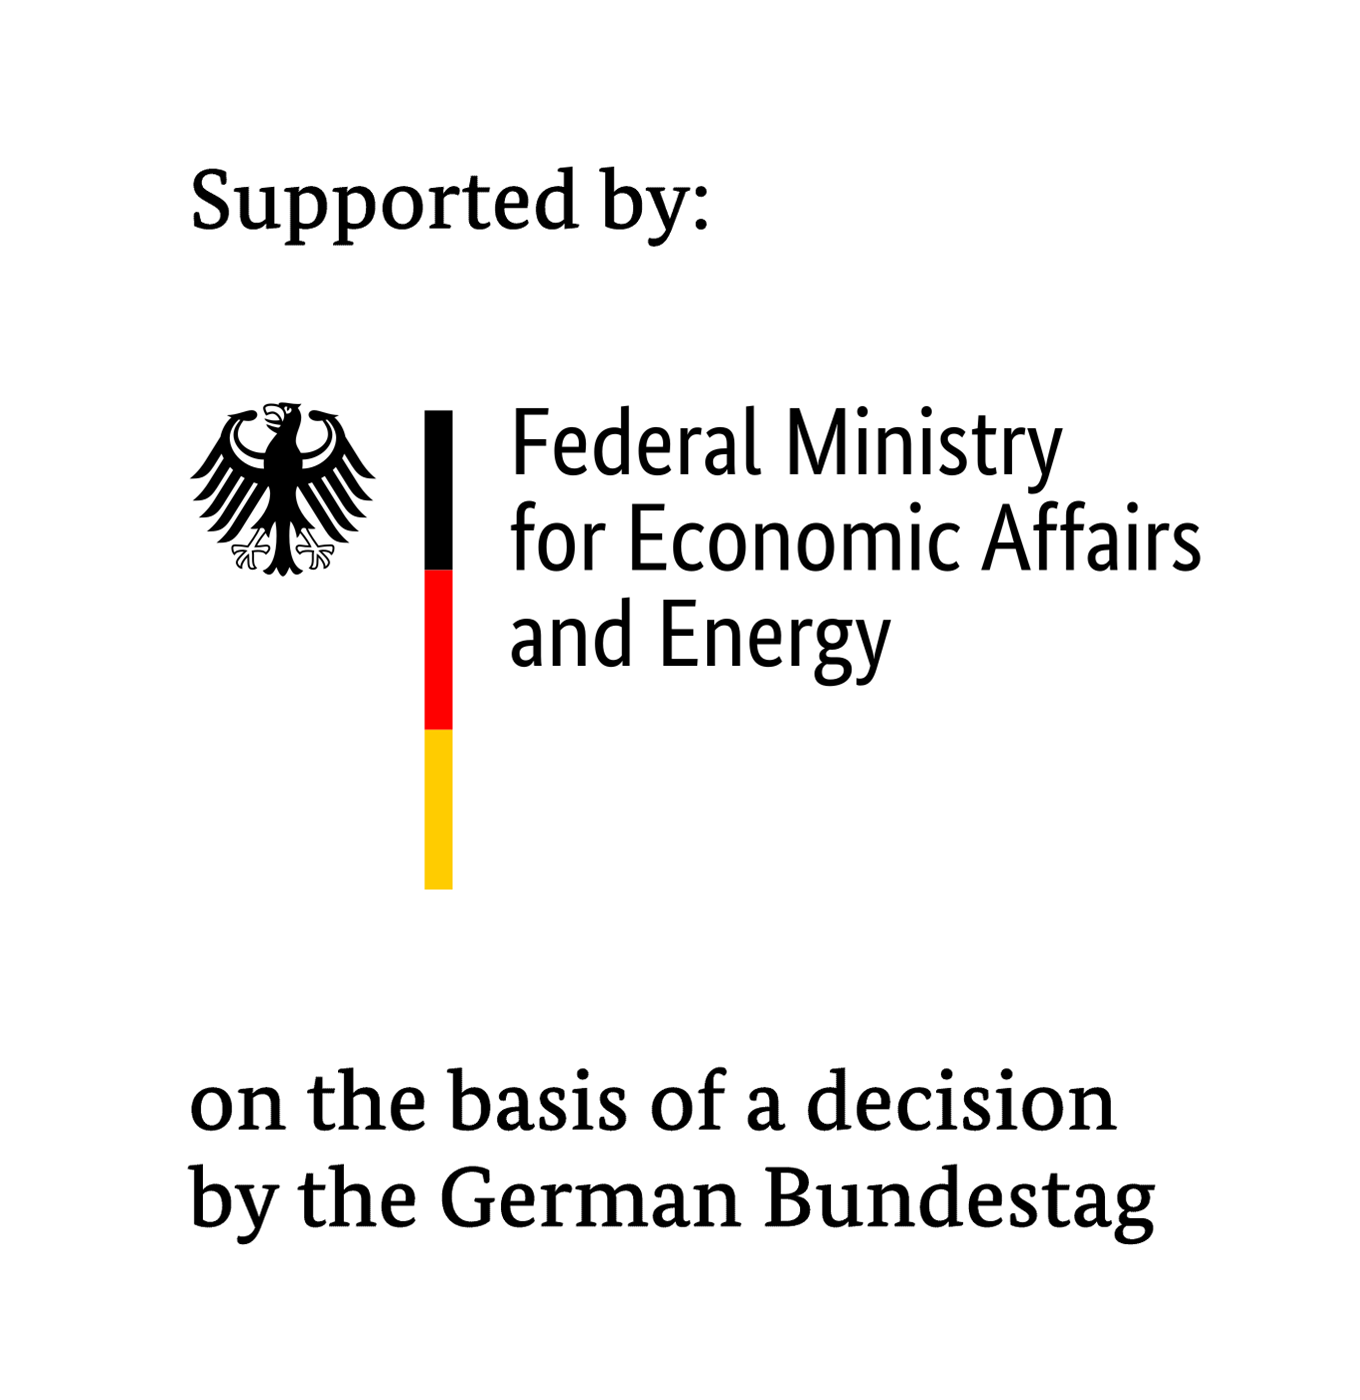
\includegraphics[trim=0.2cm 0.6cm 0.6cm 0.2cm,height=1.1cm,clip=true]{graphics/logos/bmwe_en_logo.png}
}

\begin{document}

\addtocounter{framenumber}{-1}
{
	\setbeamertemplate{footline}{
		\usebeamercolor[fg]{framesource}%
		\usebeamerfont{page number in head}%
		\begin{center}
			\Large
			\doclicenseIcon
			\vspace{0.4cm}
		\end{center}
	}
	\maketitle
}

% PROJECT CONTEXT
\section{RESILIENT}
\begin{frame}{RESILIENT project partners}
	\centering
	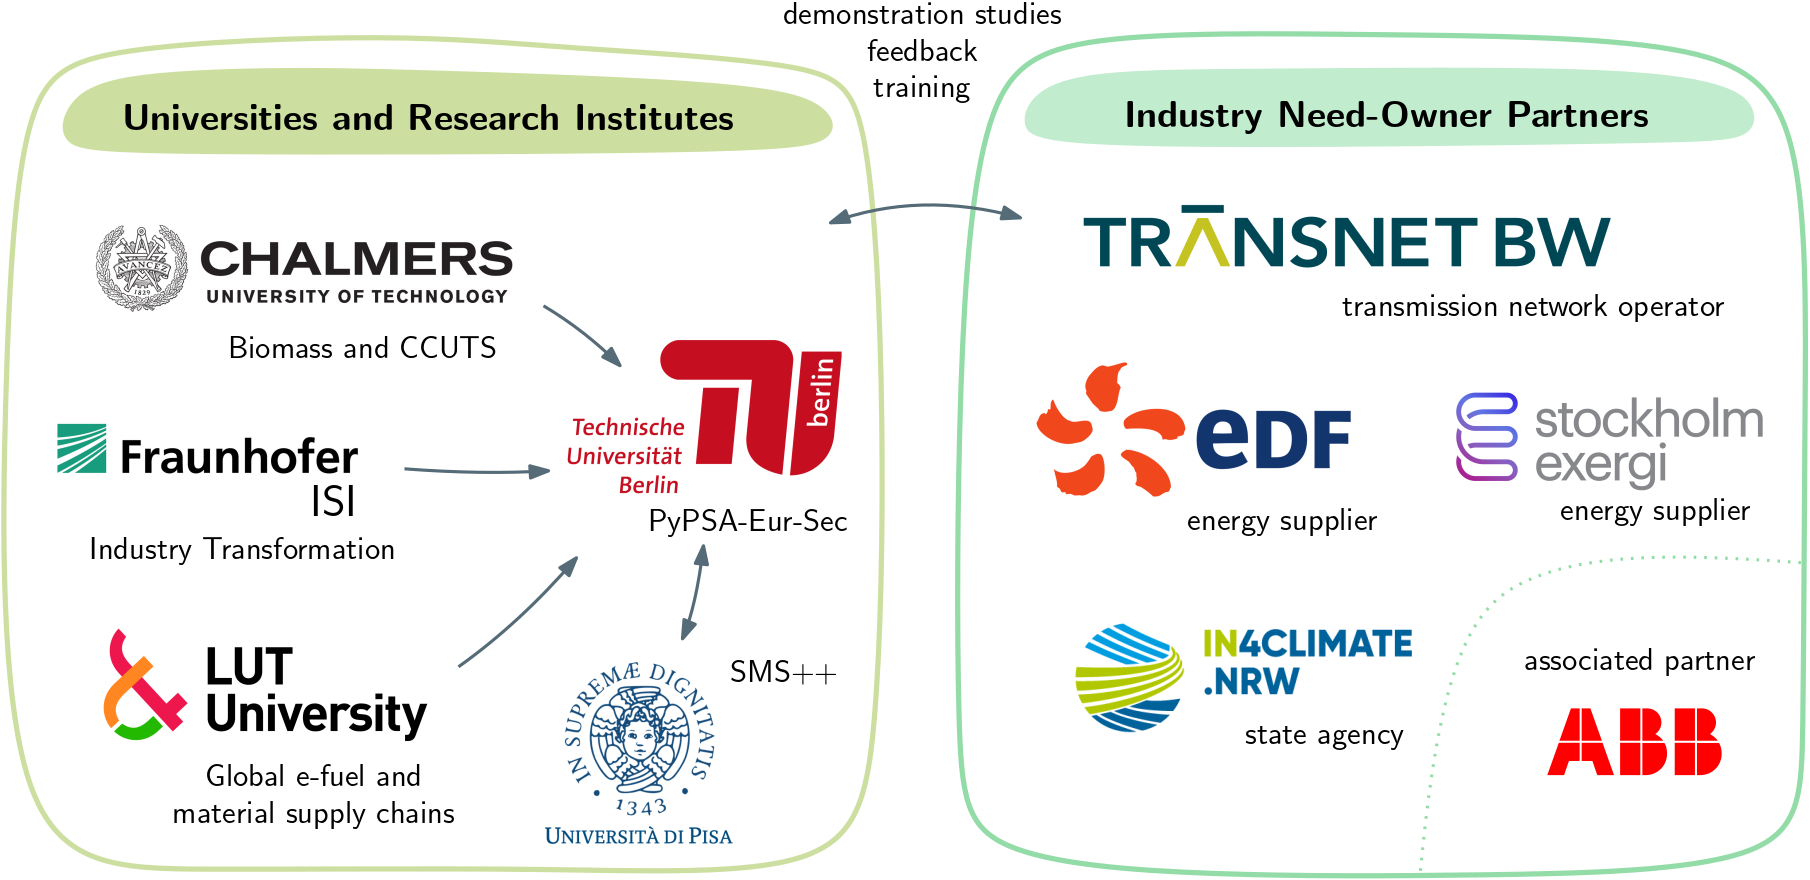
\includegraphics[width=0.85\textwidth]{graphics/resilient_partners}

	\footnotesize
	Funded through the \alert{CETPartnership 2022} call and by the \alert{German Federal Ministry for Economic Affairs and Energy (BMWE)} for the German project partners.

	\source{\url{https://resilient-project.github.io/}}
\end{frame}

\begin{frame}{Working packages}
	\centering
	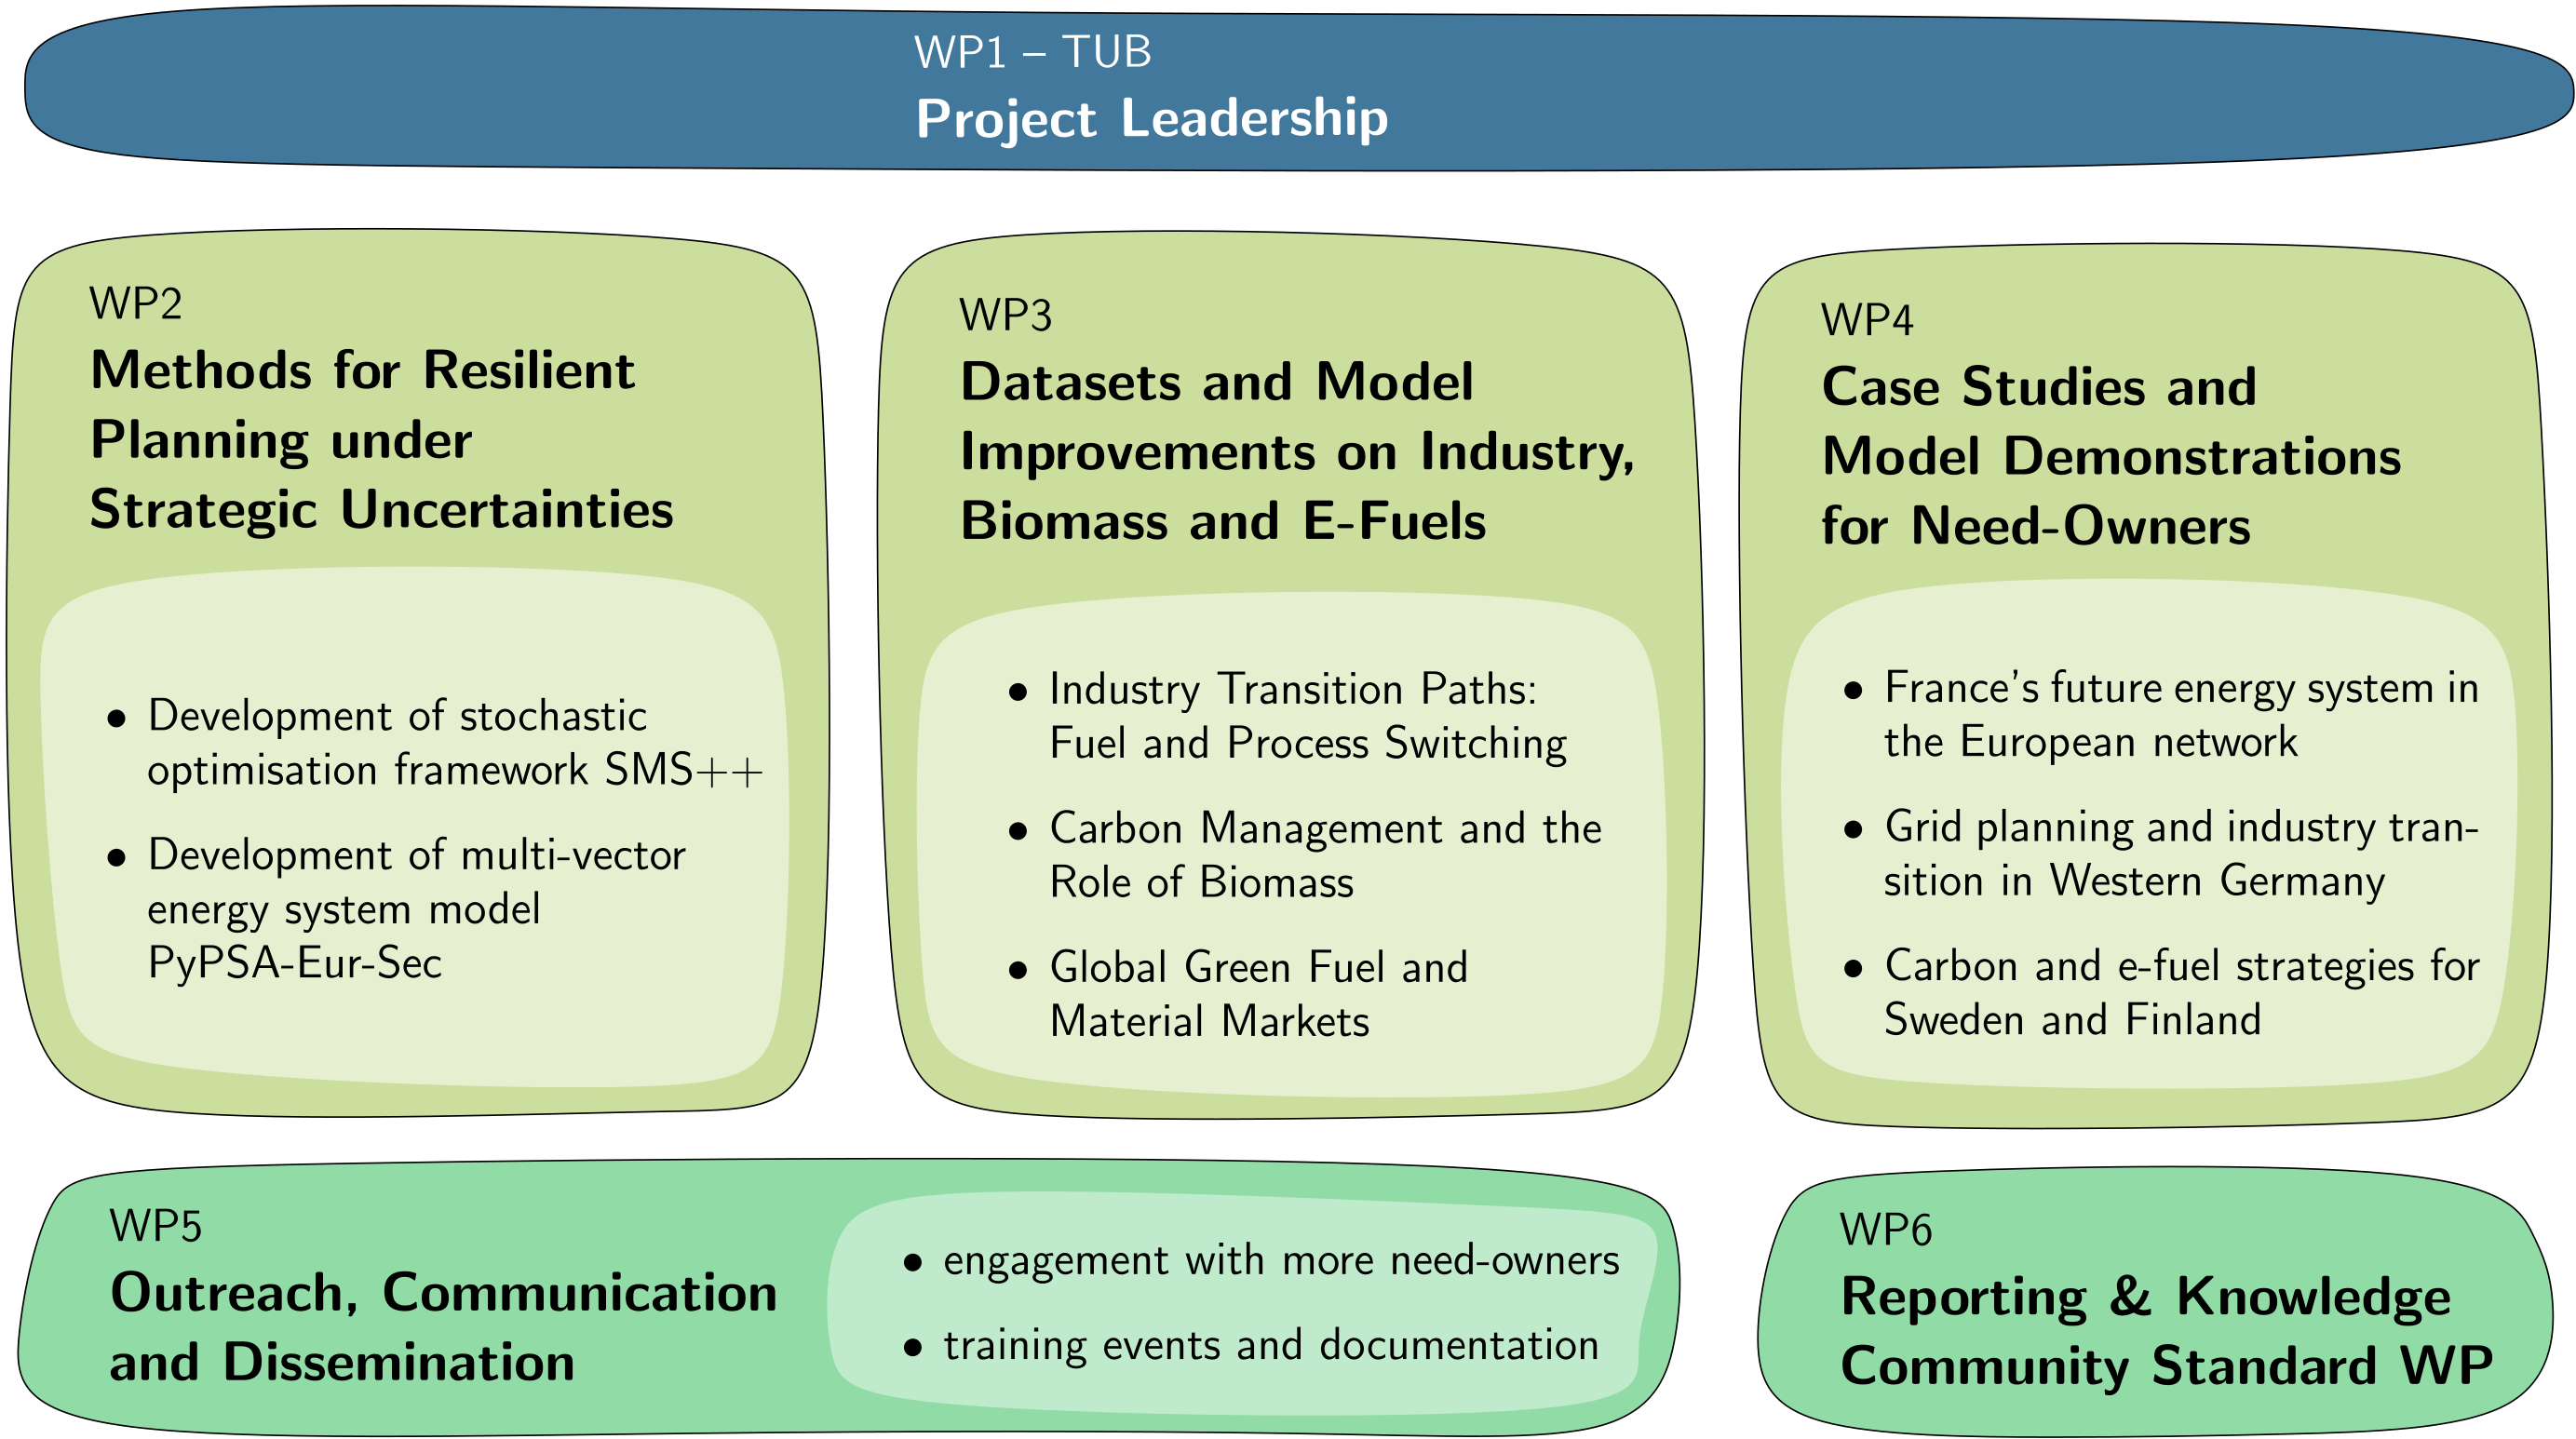
\includegraphics[width=0.8\textwidth]{graphics/resilient_project_structure}
	\source{\url{https://resilient-project.github.io/}}
\end{frame}

\section{Motivation}
 % MOTIVATION
 {\setbeamerfont{itemize/enumerate body}{size=\footnotesize}
  \begin{frame}{Motivation: the grid is no longer a given}
	  \vspace{-0.4em}
	  \begin{columns}[T,onlytextwidth]
		  \begin{column}{0.52\textwidth}
			  {\bfseries\color{adv}Recent outages and attacks in Europe}\par\smallskip
			  \begin{itemize}\setlength{\itemsep}{0.35em}
				  \item \textbf{Ukraine, since 2022:} systematic strikes on critical infrastructure, incl. generation and grid
				  \item \textbf{Baltic Sea, Oct 2023 \& Dec 2024:} Balticconnector gas pipeline and
				        Estlink~2 power cable damaged by dragged ship anchors; Estlink~2 out ${\sim}$6
				        months
				  \item \textbf{Iberia, Apr 2025:} whole peninsula blacked out, ${\sim}$10\,h to restore
				        most areas
				  \item \textbf{Berlin, Sep 2025 \& Jan 2026:} arson on high-voltage cables,
				        ${\sim}$50\,k / 45\,k households dark for 2.5 / 4 days
			  \end{itemize}
		  \end{column}
		  \begin{column}{0.44\textwidth}
			  {\bfseries\color{inv}What current planning models do}\par\smallskip
			  \begin{itemize}\setlength{\itemsep}{0.35em}
				  \item Resilience studied for \textbf{weather extremes}, Dunkelflaute events, and \textbf{fuel-import
					        disruption}
				  \item $N{-}1$ covers the instant loss of \emph{one} element
				  \item The grid itself is assumed \textbf{always available}
				        %\item EU policy asks for resilient critical entities (CER Directive 2022/2557)
			  \end{itemize}
		  \end{column}
	  \end{columns}
	  \vspace{0.3em}
	  \takeaway{\textbf{What if every region had to ride through on its own $\rightarrow$ for hours, days,
			  or weeks?}}
	  \source{ENTSO-E/ACER expert panel (2025); IEA (2026) \emph{Energy System Resilience --
			  Lessons from Ukraine}; Stromnetz Berlin (2025, 2026); Finnish NBI (2023, 2024); Fingrid (2025); Directive (EU)
		  2022/2557. Weather: Grochowicz et al.\ (2025), Bernecker et al.\ (2025). Imports: Riepin et
		  al.\ (2022), Keutz \& Kopp (2025), Göke et al.\ (2025).}
  \end{frame}}

 % RESEARCH QUESTIONS
 {\setbeamerfont{itemize/enumerate body}{size=\footnotesize}
  \begin{frame}{What does it take for every region to ride through on its own?}
	  \begin{columns}[T,onlytextwidth]
		  \begin{column}{0.56\textwidth}
			  \begin{enumerate}\setlength{\itemsep}{0.8em}
				  \item How much \textbf{more} must a net-zero German power and electrified-heat system
				        \textbf{invest} so that each region can serve its own load when \textbf{all
					        inter-regional transmission fails for 6\,h to 2~weeks}?
				  \item \textbf{Which technologies} (batteries, iron-air, hydrogen, firm capacity)
				        \textbf{and which regions} carry that resilience, and how does the mix shift as
				        outages get longer?
				  \item Can a \textbf{stored renewable methanol reserve} contribute to resilience, and how much does it \textbf{impact the cost of long outages}?
			  \end{enumerate}
		  \end{column}
		  \begin{column}{0.40\textwidth}
			  \colorbox{panel}{\parbox{\dimexpr\linewidth-2\fboxsep}{\scriptsize
					  {\bfseries Why adaptive robust optimisation?}\par\smallskip
					  \begin{itemize}\setlength{\itemsep}{0.2em}
						  \item No credible probability for \emph{when} an attack hits $\rightarrow$ plan
						        against the \textbf{worst start time}
						  \item Investment fixed before; dispatch \textbf{and storage} adapt during the outage
						  \item Worst window searched \textbf{across the whole weather year}
					  \end{itemize}
					  \vspace{0.1em}}}
		  \end{column}
	  \end{columns}
	  \source{ARO: Bertsimas et al.\ (2013); Zeng \& Zhao (2013); applied to energy planning in
		  Riepin et al.\ (2022), Bernecker et al.\ (2025).}
  \end{frame}}

\section{Method}
% METHOD (schematic built up in four steps)
\begin{frame}{Method: adaptive robust optimisation (ARO)}
	\centering\vspace*{-0.3em}
	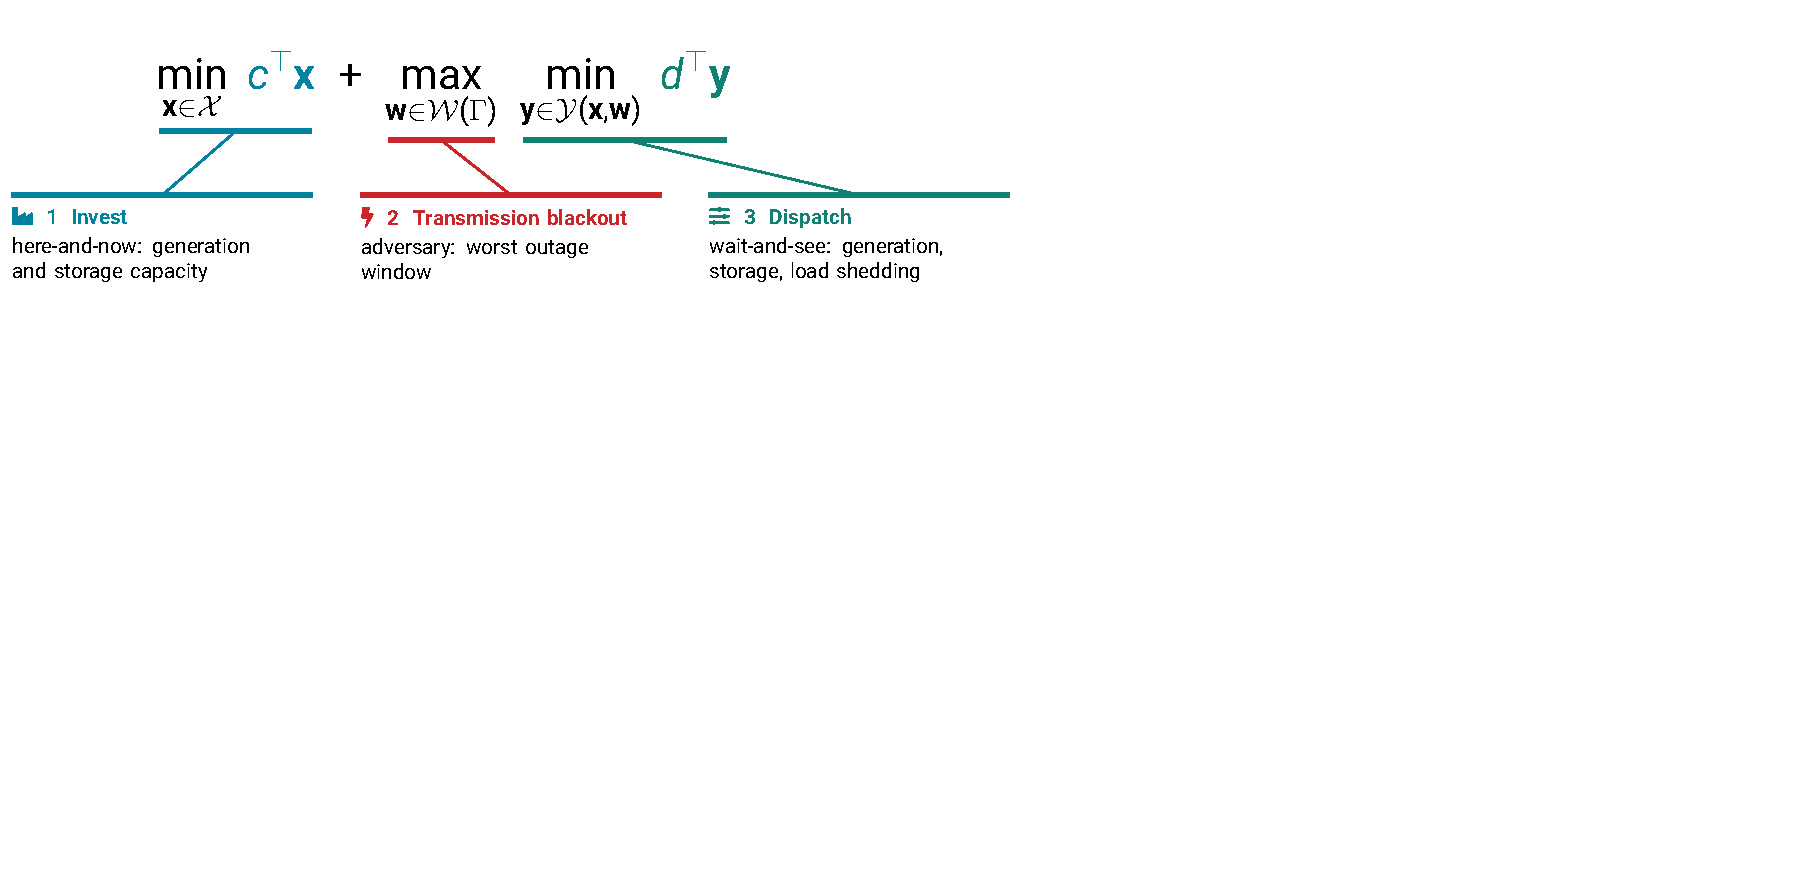
\includegraphics[width=\textwidth,height=0.86\textheight,keepaspectratio]{graphics/resilient-islands/aro-setup-step1.pdf}
\end{frame}
\begin{frame}{Method: adaptive robust optimisation (ARO)}
	\centering\vspace*{-0.3em}
	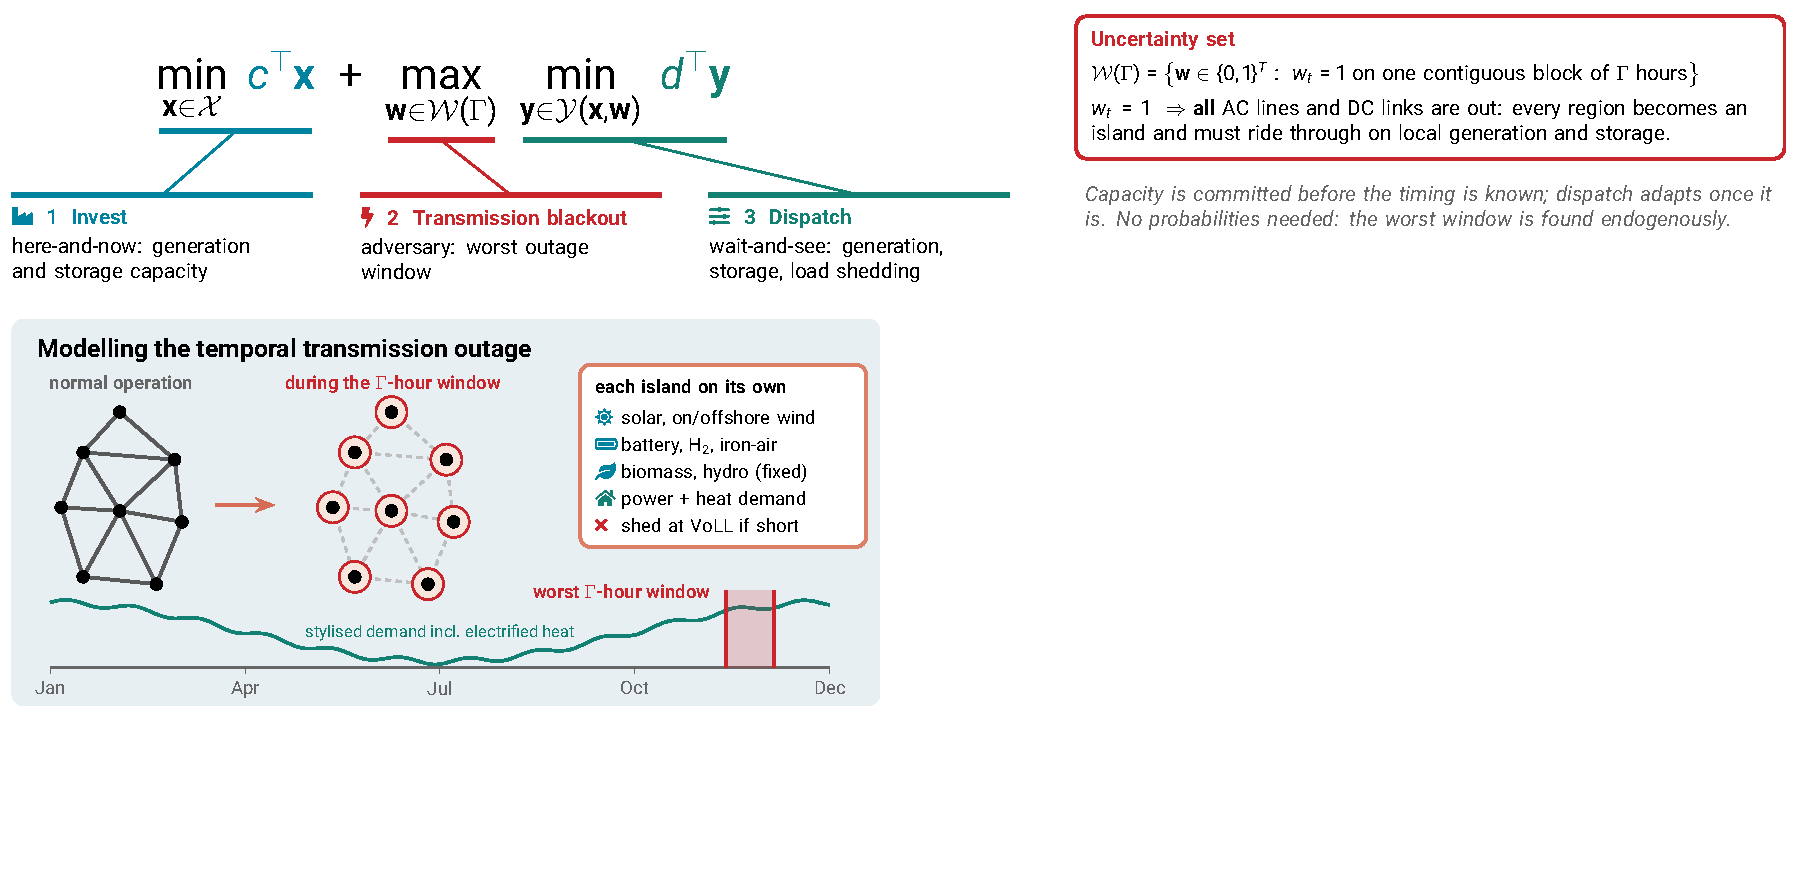
\includegraphics[width=\textwidth,height=0.86\textheight,keepaspectratio]{graphics/resilient-islands/aro-setup-step2.pdf}
\end{frame}
\begin{frame}{Method: adaptive robust optimisation (ARO)}
	\centering\vspace*{-0.3em}
	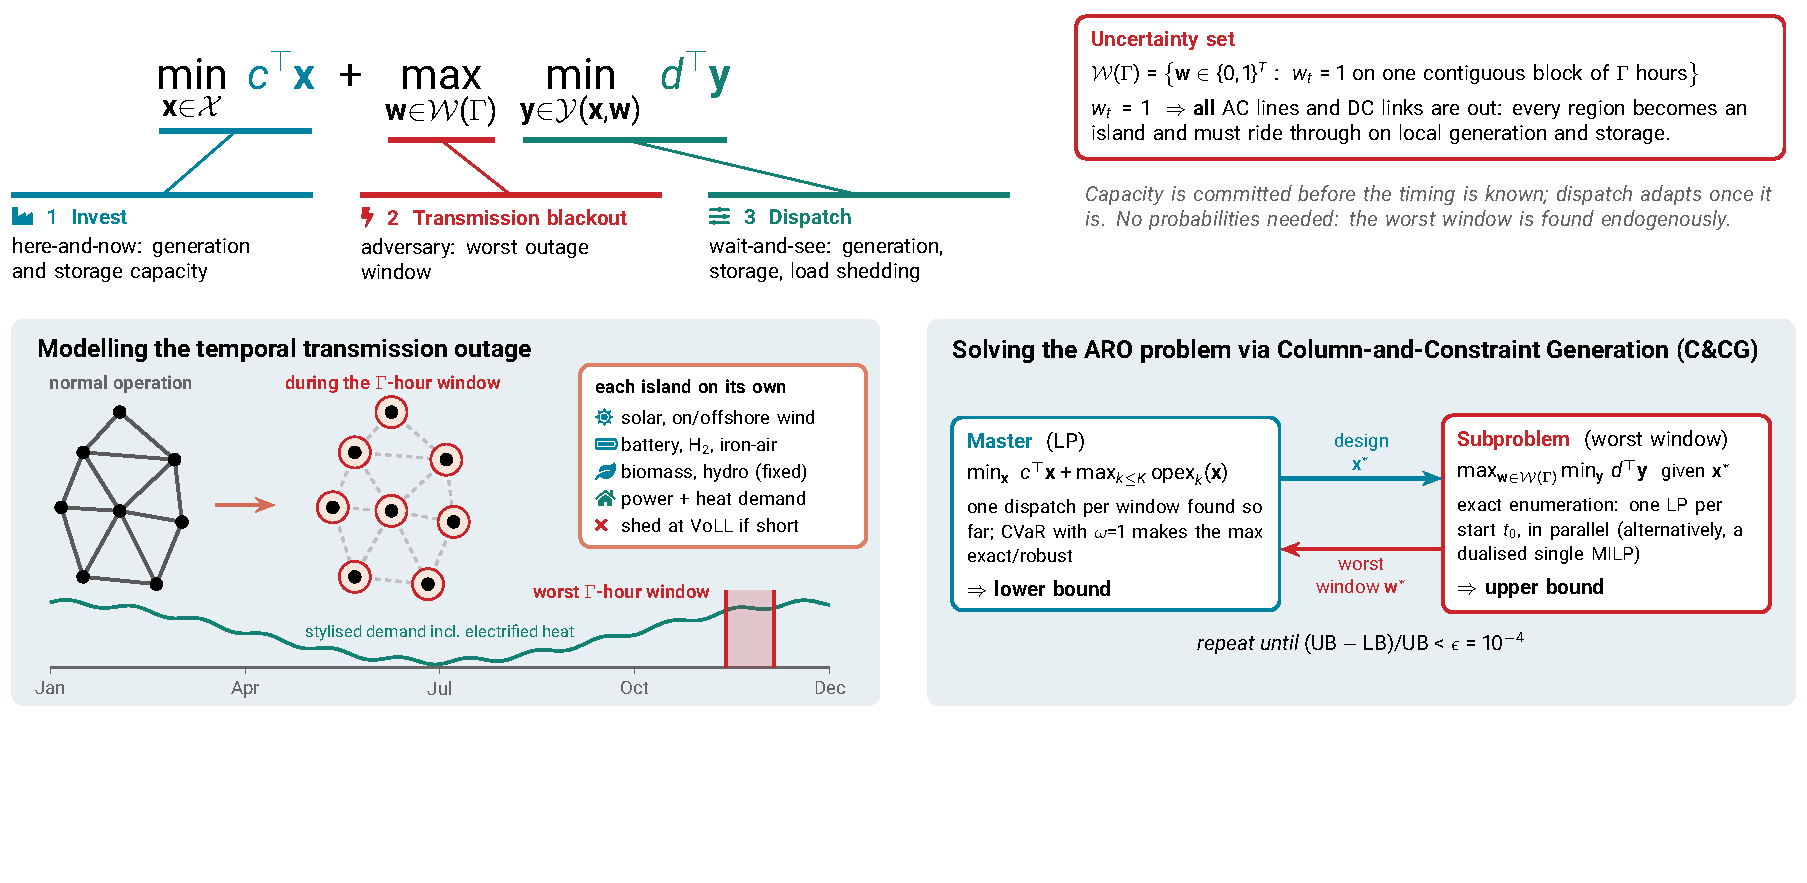
\includegraphics[width=\textwidth,height=0.86\textheight,keepaspectratio]{graphics/resilient-islands/aro-setup-step3.pdf}
\end{frame}
\begin{frame}{Method: adaptive robust optimisation (ARO)}
	\centering\vspace*{-0.3em}
	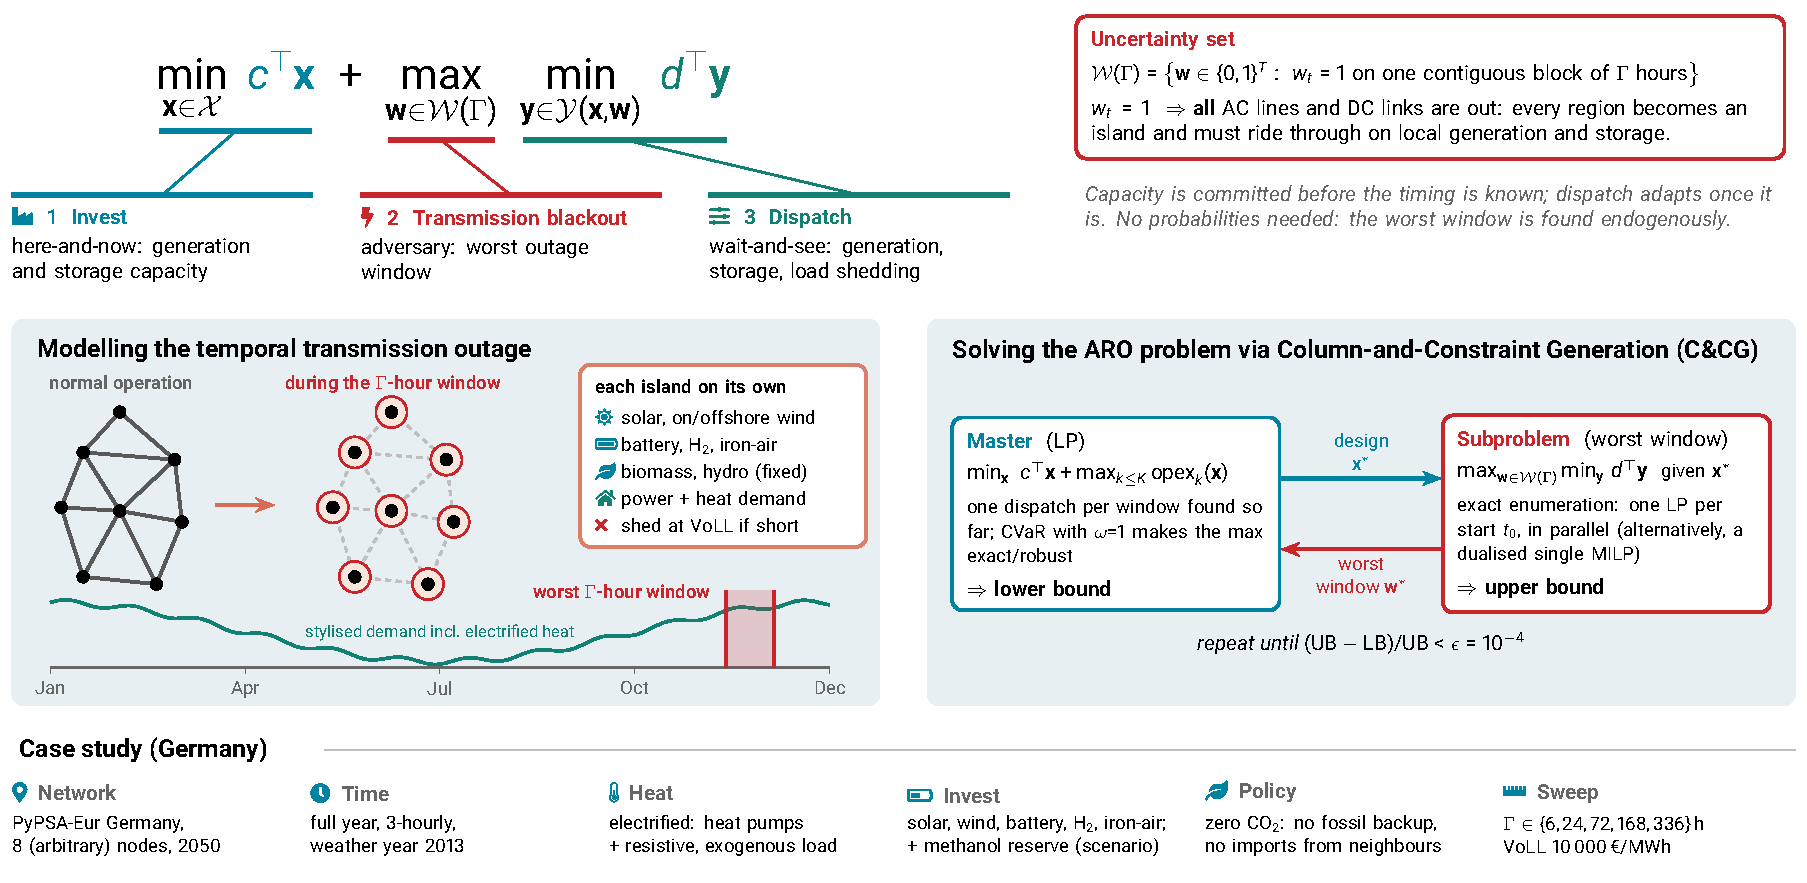
\includegraphics[width=\textwidth,height=0.86\textheight,keepaspectratio]{graphics/resilient-islands/aro-setup-step4.pdf}
\end{frame}

% PYPSA-EUR
\begin{frame}{PyPSA-Eur: A sector-coupled energy system model for Europe}
	\begin{columns}
		\begin{column}{0.5\textwidth}
			\footnotesize
			\begin{itemize}
				\setlength\itemsep{.8em}
				\item Spatially and temporally highly resolved linear optimisation model covering the \alert{European continent},
				\item Based on the open-source framework \alert{PyPSA},
				\item Includes \alert{existing power plant fleet}, \alert{renewable potentials}, and \alert{availability time series},
				\item Includes the \alert{electrical transmission grid} from 220 kV to 750 kV (AC, including Ukraine) and from 150 kV (DC), with the option to enable planned grid expansion projects (TYNDP and German NEP), as well as the gas network,
				\item Maintained by the Department of Digital Transformation in Energy Systems at \alert{TU Berlin}.
			\end{itemize}
		\end{column}
		\begin{column}{0.5\textwidth}
			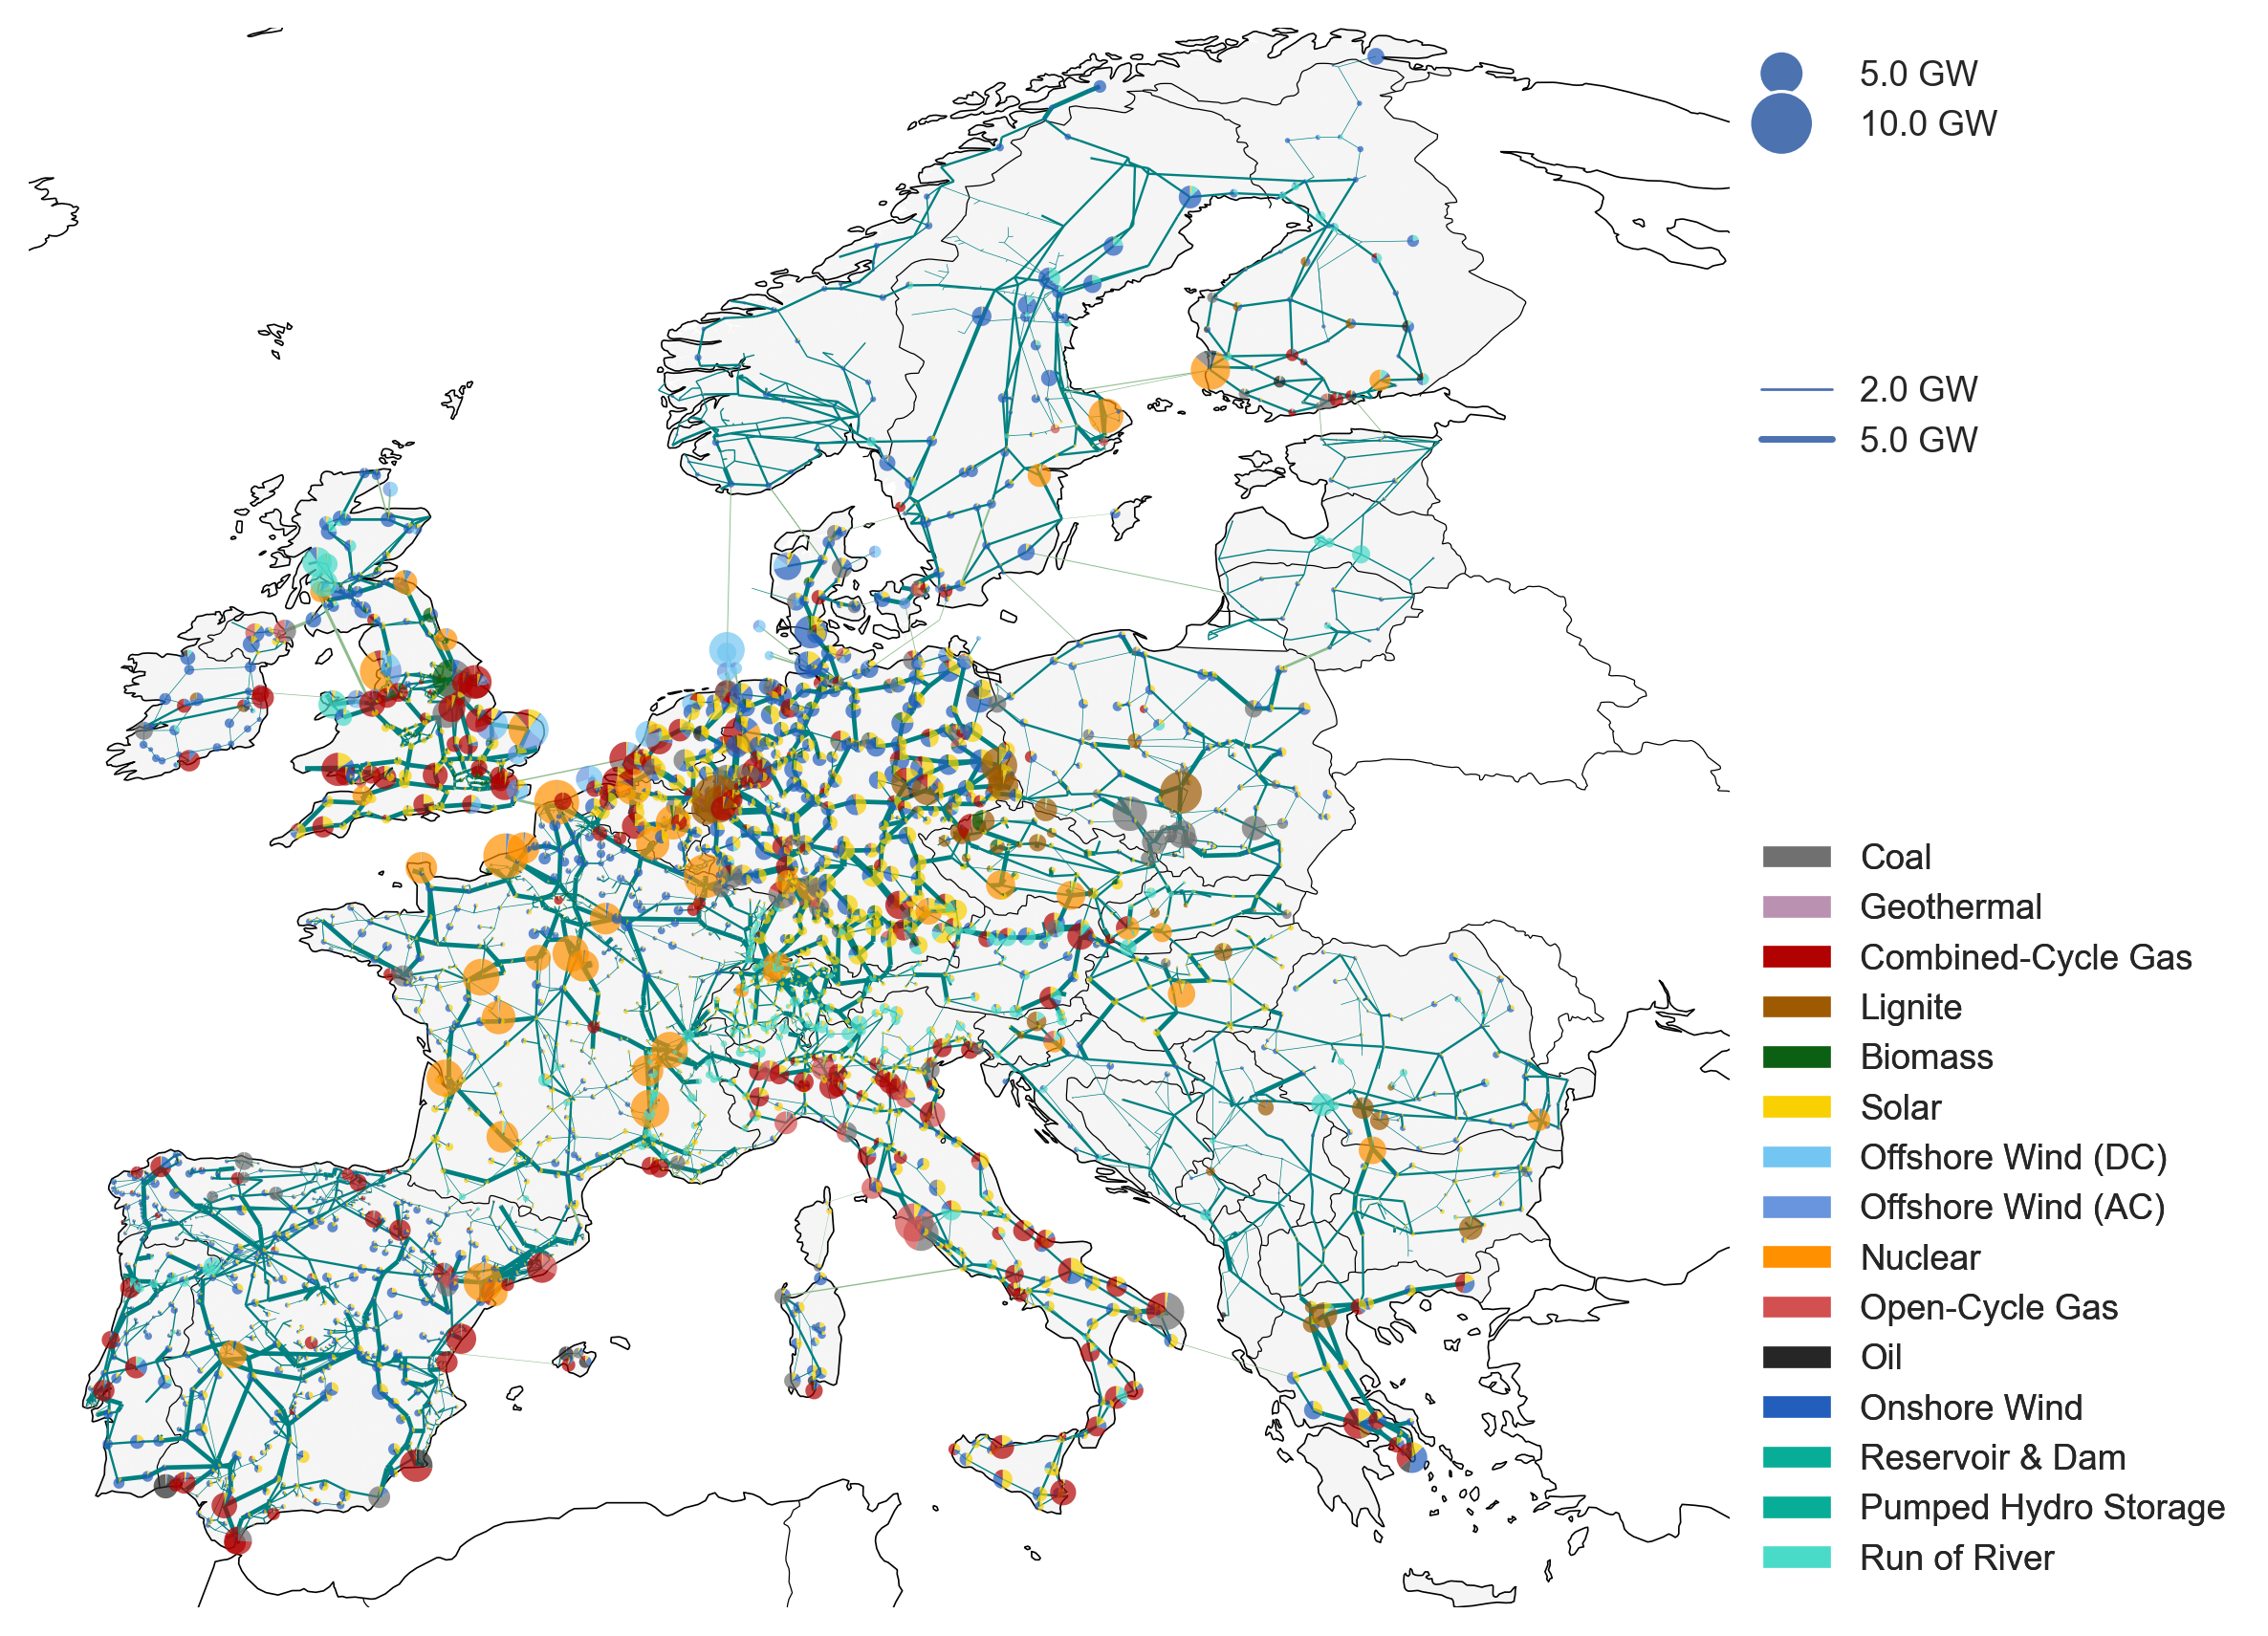
\includegraphics[width=1\textwidth]{graphics/pypsa_eur_elec}
		\end{column}
	\end{columns}

	\source{\url{https://pypsa-eur.readthedocs.io}}
\end{frame}

% HEDGE OPTIONS
{\setbeamerfont{itemize/enumerate body}{size=\small}
\begin{frame}{Two scenarios: storage only, or storage plus a methanol reserve}
	\begin{columns}[T,onlytextwidth]
		\begin{column}{0.36\textwidth}
			\begin{itemize}\setlength{\itemsep}{0.5em}
				\item \textbf{No methanol:} battery, iron-air, H$_2$ (caverns where geology allows + local tanks)
				\item \textbf{Methanol:} additionally buy renewable methanol at
				      130\,\texteuro/MWh, store it in local tanks, burn it in turbines \emph{only
					      during an outage}
				\item Holding fuel in tanks is cheap; turbine capacity is not. Long outages favour
				      \textbf{cheap energy, expensive power}
			\end{itemize}
		\end{column}
		\begin{column}{0.62\textwidth}
			\centering
			\includegraphics[width=\linewidth,height=0.72\textheight,keepaspectratio]{%
				graphics/resilient-islands/backup_cost_by_duration.png}\par\smallskip
			{\raggedright\scriptsize\color{mute}
				Standalone sizing for 1\,MW over $\Gamma$ hours, outage once a year. Running cost =
				purchased methanol + VOM. \textbf{Not included:} electricity to recharge storage or
				make H$_2$ (round-trip losses, electrolyser), shared with normal operation and paid
				in the optimisation.\par}
		\end{column}
	\end{columns}
	\source{Costs from the model's cost assumptions. Methanol price: Wenzel et al.\ (2026);
		minimal methanol economy: Glaum et al.\ (2025).}
\end{frame}}

\section{Results}
% RESULTS: no methanol
\begin{frame}{Storage can secure multi-day autonomy for +0.3--12.4\,\%}
	\centering
	\vspace{-0.4em}
	\includegraphics[width=\linewidth,height=0.80\textheight,keepaspectratio]{%
		graphics/resilient-islands/robust_design_slides_no-methanol.png}
	\takeaway{Batteries cover hours, \textbf{iron-air} takes over beyond 3 days (+61\,GW at
		336\,h); from there, each extra day of autonomy adds a steady ${\sim}$0.7\,bn\texteuro/a.}
\end{frame}

% RESULTS: methanol
\begin{frame}{Methanol-based backup makes long outages cheaper to survive}
	\centering
	\vspace{-0.4em}
	\includegraphics[width=\linewidth,height=0.72\textheight,keepaspectratio]{%
		graphics/resilient-islands/robust_design_slides_methanol.png}
	\takeaway{Two weeks of autonomy for \textbf{+3.8\,\%} instead of +12.4\,\% with storage
		alone. Identical up to 24\,h; from 72\,h on, methanol turbines replace iron-air and each
		extra hour only adds fuel to the tank (19\,TWh at 336\,h).}
	\source{Costs: all installed capex + no-outage opex; fuel burned during the event excluded. 336\,h is the
		best design after 9 C\&CG iterations (gap 0.08\,\% of total cost); all other points
		converged.}
\end{frame}

% RESULTS: marginal cost of resilience
{\setbeamerfont{itemize/enumerate body}{size=\scriptsize}
\begin{frame}{What one more hour of autonomy costs}
	\centering
	\vspace{-0.2em}
	\includegraphics[width=\linewidth,height=0.82\textheight,keepaspectratio]{%
		graphics/resilient-islands/marginal_cost_comparison.png}
	\takeaway{First day: ${\sim}$37\,M\texteuro/a per outage hour (batteries). Beyond 3 days:
		${\sim}$28 with storage alone (iron-air) vs.\ 3--5 with methanol (${\sim}$11 incl.\ one
		outage's fuel a year), i.e.\ each extra day costs \textbf{${\sim}$0.7} vs.\
		\textbf{0.1--0.3\,bn\texteuro/a}.}
	\source{Top: $\mathrm{d}C/\mathrm{d}\Gamma$ at each modelled $\Gamma$ (central
		differences). Bottom: total system cost (all installed capex + no-outage opex). Red: fuel
		\& shedding if the outage happens once a year.}
\end{frame}}

% RESULTS: regional
\begin{frame}{Islands need local supply, resilience moves south}
	\vspace{-0.3em}
	\begin{columns}[T,onlytextwidth]
		\begin{column}{0.79\textwidth}
			\centering
			\includegraphics[width=\linewidth,height=0.84\textheight,keepaspectratio]{%
				graphics/resilient-islands/regional_capacity_map_methanol.png}
		\end{column}
		\begin{column}{0.20\textwidth}
			\vspace{4.5em}
			\colorbox{panel}{\parbox{\dimexpr\linewidth-2\fboxsep}{\scriptsize\raggedright
					\textbf{German case study:}\par\smallskip
					Onshore wind leaves the Northwest; solar shifts from the north to Hesse and
					Bavaria.\par\medskip
					Batteries move south for short outages only.\par\medskip
					The methanol reserve sits only in the south, where there are no salt caverns
					for H$_2$.\par}}
		\end{column}
	\end{columns}
\end{frame}

\section{Discussion}
 % DISCUSSION
 % payback = (worst-case opex saved) / (extra capex); robust designs have foresight,
 % so this is a pessimistic bound
 {\setbeamerfont{itemize/enumerate body}{size=\footnotesize}
  \begin{frame}{Limitation: the hedge pays off if storage is held in reserve}
	  \begin{columns}[T,onlytextwidth]
		  \begin{column}{0.47\textwidth}
			  {\scriptsize
				  \setlength{\tabcolsep}{2.5pt}
				  \begin{tabular}{@{}r c c c@{}}
					  \toprule
					           & capex premium   & \multicolumn{2}{c}{payback = avoided damage\,/\,premium}                                \\
					  \cmidrule(l){3-4}
					  $\Gamma$ & bn\,\texteuro/a & with foresight                                           & \textbf{no foresight}        \\
					  \midrule
					  6\,h     & 0.29            & 8$\times$                                                & \textbf{1.1$\times$}         \\
					  24\,h    & 1.14            & 10$\times$                                               & \textbf{1.6$\times$}         \\
					  \midrule
					  \multicolumn{4}{@{}l}{\color{mute}no methanol\,/\,methanol}                                                          \\
					  72\,h    & 2.1\,/\,2.0     & 15\,/\,16$\times$                                        & \textbf{5.5\,/\,8.1$\times$} \\
					  168\,h   & 4.9\,/\,2.5     & 15\,/\,29$\times$                                        & \textbf{6.4\,/\,22$\times$}  \\
					  336\,h   & 9.9\,/\,3.0     & 15\,/\,48$\times$                                        & \textbf{8.0\,/\,36$\times$}  \\
					  \bottomrule
				  \end{tabular}}
			  \par\medskip
			  {\scriptsize\color{mute} Robust design vs.\ the non-robust design, re-evaluated over
				  all outage windows with storage levels fixed at the outage start.\par}
		  \end{column}
		  \begin{column}{0.46\textwidth}
			  \begin{itemize}\setlength{\itemsep}{0.4em}
				  \item The model sizes and \textbf{pre-charges storage} knowing when the outage starts
				  \item Short $\Gamma$: without foresight the premium barely pays back (1.1--1.6$\times$), but it is also small (0.3--1.1\,bn\texteuro/a), so
				        little is at stake
				  \item Long $\Gamma$: robustness \textbf{survives}, still 5--36$\times$ payback
				  \item A held \textbf{fuel reserve is more resilient}, e.g. the methanol design is the most foresight-proof
			  \end{itemize}
		  \end{column}
	  \end{columns}
  \end{frame}}

 % MAIN FINDINGS
 {\setbeamerfont{itemize/enumerate body}{size=\small}
  \begin{frame}{Main findings}
	  \vspace{-0.4em}
	  \begin{enumerate}\setlength{\itemsep}{0.55em}
		  \item \textbf{Up to 3 days, resilience is cheap:} +0.3\,\% (6\,h), +1.3\,\% (24\,h),
		        +2.3--2.5\,\% (72\,h) of system cost --- 0.2 to 1.9\,bn\texteuro/a.
		  \item \textbf{Beyond 3 days, the hedge decides the bill:} two weeks cost
		        \textbf{+12.4\,\%} (9.4\,bn\texteuro/a) with storage alone, \textbf{+3.8\,\%}
		        (2.9\,bn\texteuro/a) with a methanol reserve --- 5.2\,bn\texteuro/a if the
		        fuel of one outage per year is counted.
		  \item \textbf{The cheapest hedge changes with duration:} batteries for hours, iron-air for
		        days, a fuel stock for weeks. The stock scales with turbine capacity $\times\,\Gamma$
		        (19\,TWh at 2 weeks), so each extra hour only adds fuel.
		  \item \textbf{Resilience is local:} islands need supply where the load is, in the case of Germany, onshore wind leaves the Northwest, solar and the methanol reserve go south.
		  \item \textbf{Storage levels at the outage start matter:} with sufficient reserves
		        held, robust designs pay back many times over for outages beyond 3 days, most of all with the methanol reserve.
	  \end{enumerate}
	  \source{Preliminary: German 8-region case, one weather year; costs exclude fuel burned during
		  the outage.}
  \end{frame}}

 % POLICY (oil stock analogy: Council Directive 2009/119/EC, 90 days)
 {\setbeamerfont{itemize/enumerate body}{size=\small}
  \begin{frame}{What this means for European (German) energy policy}
	  \begin{enumerate}\setlength{\itemsep}{0.7em}
		  \item \textbf{Set an explicit resilience target:} name the outage duration to plan for.
		        The cost curve prices each extra day.
		  \item \textbf{Regulate reserves, do not leave them (fully) to the market:} resilient capacity only
		        pays off if it is held in reserve, i.e. a storage obligation, like the EU's 90-day oil
		        stocks.
		  \item \textbf{Recognise strategic fuel reserves,} e.g.\ methanol: the cheapest hedge beyond
		        ${\sim}$3 days where there are no H$_2$ caverns
		  \item \textbf{Plan resilience regionally:} firm capacity near load, alternatives where
		        there are no H$_2$ caverns.
		  \item \textbf{Stress-test grid loss} in adequacy assessments (ERAA, TYNDP), next to
		        weather extremes.
	  \end{enumerate}
	  \source{Preliminary: German 8-region case, one weather year. Oil stocks: Council Directive
		  2009/119/EC. Risk assessments of critical entities: Directive (EU) 2022/2557.}
  \end{frame}}

\section{Outlook}
 % OUTLOOK
 {\setbeamerfont{itemize/enumerate body}{size=\small}
  \begin{frame}{Outlook}
	  \begin{itemize}\setlength{\itemsep}{0.8em}
		  \item \textbf{Scale to Europe:} 156 NUTS1/2 regions; each country plans against its own
		        worst case, border flows from a European pre-run
		  \item \textbf{Several weather years}, VoLL sensitivity, finer regions
		  \item Cost sensitivities on methanol
		  \item (\textbf{Future work outside this scope}) \textbf{Non-anticipative recourse:} stays two-stage, because only the outage \emph{onset} is uncertain
	  \end{itemize}
	  \vspace{1em}
	  \takeaway{\centering How much resilience does Europe need, and how much does it cost?}
  \end{frame}}

\begin{frame}
	\setbeamercolor{background canvas}{bg=red}
	\centering
	\fcolorbox{white}{tub-red}{\parbox[c][0.9\textheight][c]{\textwidth}{%
			\centering \color{white}\Large{\textbf{Thank you.}} \\
			\scriptsize
			\vspace{0.5cm}
			\textbf{The cost of self-sufficiency} \\
			\textit{Robust energy system planning under prolonged transmission blackouts} \\
			\vspace{0.5cm}
			Bobby Xiong, Iegor Riepin, Tom Brown \\
			\href{mailto:xiong@tu-berlin.de}{\textcolor{white}{$\hookrightarrow$ xiong@tu-berlin.de}} \\
			\vspace{0.5cm}
			Department of\\\textbf{Digital Transformation in Energy Systems (ENSYS)} \\
			Technische Universität Berlin
		}}
\end{frame}

% BACKUP
\appendix

\section{Backup}

 % Caveats
 {\setbeamerfont{itemize/enumerate body}{size=\small}
  \begin{frame}{Backup: caveats}
	  \begin{itemize}\setlength{\itemsep}{0.7em}
		  \item \textbf{Controlled islanding}, not black start: regions stay energised; restart after
		        a collapse is out of scope and strictly worse
		  \item 8 regions: islands far larger than reality $\Rightarrow$ premium likely a
		        \textbf{lower bound}
		  \item One weather year (2013), 3-hourly; no imports from neighbours
		  \item VoLL 10\,000\,\texteuro/MWh; heat as an inflexible load
		  \item Reported costs exclude the outage's own running cost. Counting the fuel burned in
		        one outage per year shrinks methanol's advantage at 2 weeks from 3.3$\times$ to
		        ${\sim}$1.9$\times$ (premium 5.2 vs 9.7\,bn\texteuro/a; red on the
		        marginal-cost slide)
	  \end{itemize}
  \end{frame}}

\begin{frame}{Backup: regional capacity incl.\ H$_2$ storage}
	\centering
	\vspace{-0.4em}
	\includegraphics[width=\linewidth,height=0.86\textheight,keepaspectratio]{%
		graphics/resilient-islands/regional_capacity_map_h2_methanol.png}
\end{frame}

\begin{frame}{Backup: dispatch in the worst window (methanol)}
	\centering
	\includegraphics[width=\linewidth,height=0.84\textheight,keepaspectratio]{%
		graphics/resilient-islands/outage_dispatch_methanol.png}
\end{frame}

{\setbeamerfont{itemize/enumerate body}{size=\tiny}
\begin{frame}{Backup: references}
	\begin{columns}[T,onlytextwidth]
		\begin{column}{0.49\textwidth}
			\begin{itemize}\setlength{\itemsep}{0.15em}
				\item Bernecker et al.\ (2025). Adaptive robust optimization for European electricity
				      system planning considering regional Dunkelflaute events. SSRN 5361178.
				\item Bertsimas et al.\ (2013). Adaptive robust optimization for the security constrained
				      unit commitment problem. \emph{IEEE Trans.\ Power Syst.}\ 28(1), 52--63.
				\item Council Directive 2009/119/EC on maintaining minimum stocks of crude oil and/or
				      petroleum products.
				\item Directive (EU) 2022/2557 on the resilience of critical entities.
				\item Expert Panel on the Grid Incident on 28 April 2025, ACER, ENTSO-E (2025). Grid
				      incident in Spain and Portugal on 28 April 2025 -- Factual report.
				\item Fingrid (2025). EstLink~2 electricity transmission link returns to commercial use,
				      press release of 18 Jun 2025.
				\item Finnish National Bureau of Investigation (2023, 2024). Balticconnector and Estlink~2
				      investigations, press statements of Oct--Nov 2023 and 26--30 Dec 2024.
				\item Glaum, Neumann, Millinger, Brown (2025). The minimal methanol economy as a
				      gap-filler for high electrification scenarios. arXiv:2505.09277.
			\end{itemize}
		\end{column}
		\begin{column}{0.49\textwidth}
			\begin{itemize}\setlength{\itemsep}{0.15em}
				\item Göke, Wohland, Moret, Bardow (2025). The liquid buffer: multi-year storage for
				      defossilization and energy security under climate uncertainty. arXiv:2511.13513.
				\item Grochowicz, Bloomfield, Victoria (2025). Preparing for the worst: long-term and
				      short-term weather extremes in resource adequacy assessment. arXiv:2508.05163.
				\item International Energy Agency (2026). Energy system resilience -- Lessons learned from
				      Ukraine.
				\item Keutz, Kopp (2025). The cost of security: analyzing strategies to hedge hydrogen
				      import disruption under stochastic representation of weather. EWI.
				\item Riepin, Schmidt, Baringo, Müsgens (2022). Adaptive robust optimization for European
				      strategic gas infrastructure planning. \emph{Appl.\ Energy} 324, 119686.
				\item Stromnetz Berlin (2025, 2026). Press releases on the Johannisthal (9--11 Sep 2025)
				      and Lichterfelde (3--7 Jan 2026) outages.
				\item Wenzel et al.\ (2026). Direct air capture enables sustainable methanol production in
				      water-scarce regions. \emph{Nature Communications} 17, 8495.
				\item Zeng, Zhao (2013). Solving two-stage robust optimization problems using a
				      column-and-constraint generation method. \emph{Oper.\ Res.\ Lett.}\ 41(5), 457--461.
			\end{itemize}
		\end{column}
	\end{columns}
\end{frame}}

\end{document}
